\chapter{Analyse de la méthode JFNK dans CEDRE}

  \paragraph{}
  In a previous chapter, we identified some methods from the literature that we wanted to use in our solver CEDRE, and some others from CEDRE that we wanted to improve.
  In another chapter, we discussed the practical implementation of said methods in the solver.
  The goal of this chapter is now to test those methods on several applications to comment on the choices we made.
  We need to define test cases that represent well enough target applications so we can comment on the performances of our choices.


  \section{Comparaison entre la matrice jacobienne explicite et la formulation sans matrice}

    \paragraph{}
    From our analysis and implementation, the main addition to the solver is the Jacobian-Free Newton--Krylov method, and in particular the matrix-free approach.
    In this part, we will then compare two methods: the traditional method and the new one that uses the matrix-free approach.
    As we are interested in implicit time integration, we will use the implicit Euler method, for reasons previously discussed.
    The traditional method linearises the equation that the implicit Euler method produces, approximates the Jacobian matrix using the Jacobian matrix of the corresponding first-order scheme, and then solves the linear system with the Krylov subspace method GMRES.
    As we want to understand the impact of a better Jacobian matrix, we are only going to change how it is computed.
    The new method will then work in a similar way, except the matrix used in the linear solver is not actually computed, but the matrix-vector products are approximated using equation (\ref{eq:matrix_free}).


    \subsection{Turbulent transonic airfoil}

      \subsubsection{Definition of the test case}

        \paragraph{}
        Our first application is a typical aerodynamics test case.
        It is a 2D simulation of the flow around an RAE 2822 wing profile.
        The only fluid is standard air.
        The Mach number is taken equal to 0.75, the chord is equal to $1\si{\meter}$, the angle of attack is $0\si{\degree}$ and we use the atmospheric conditions at 10km.
        This gives a laminar Reynolds number of \num{6.5e6}.

        \paragraph{}
        We decided to use this first test case for multiple reasons.
        Firstly, it is a simple case in the field of computational fluid dynamics.
        It is a standard aerodynamics case, with a small mesh in comparison to many other 3D cases.
        This allows us to test out methods inexpensively.
        Secondly, this case belongs to the tutorial suite of our solver.
        It means that it is already well mastered by the team.
        Thirdly, even if it is only a standard aerodynamics case it still has some stiff features, such as turbulence modelling and a shock.
        Finally, it is a standard test case for turbulence modelling validation.
        Therefore there are many references in the literature using this case.
        Even if this thesis aims at multiphysics, it is often good to start slow, and that is what we are doing with this test case.

        \paragraph{}
        The mesh used for this simulation is an unstructured hybrid mesh made of triangles and quadrangles.
        Parts of it can be seen in figure \ref{fig:rae_mesh}.
        Cell sizes range from $2.5\si{\meter}$ far from the airfoil and $100\si{\micro\meter}$ at the wall.
        At the wall, there is a C-shaped layer of regular cells.
        This helps better capture boundary layer effects near the profile and the wake.
        Also, under those conditions, a shock is expected to develop on the upper part.
        Special treatment such as refinement was applied to the mesh at the expected shock location.

        \begin{figure}
          \centering
          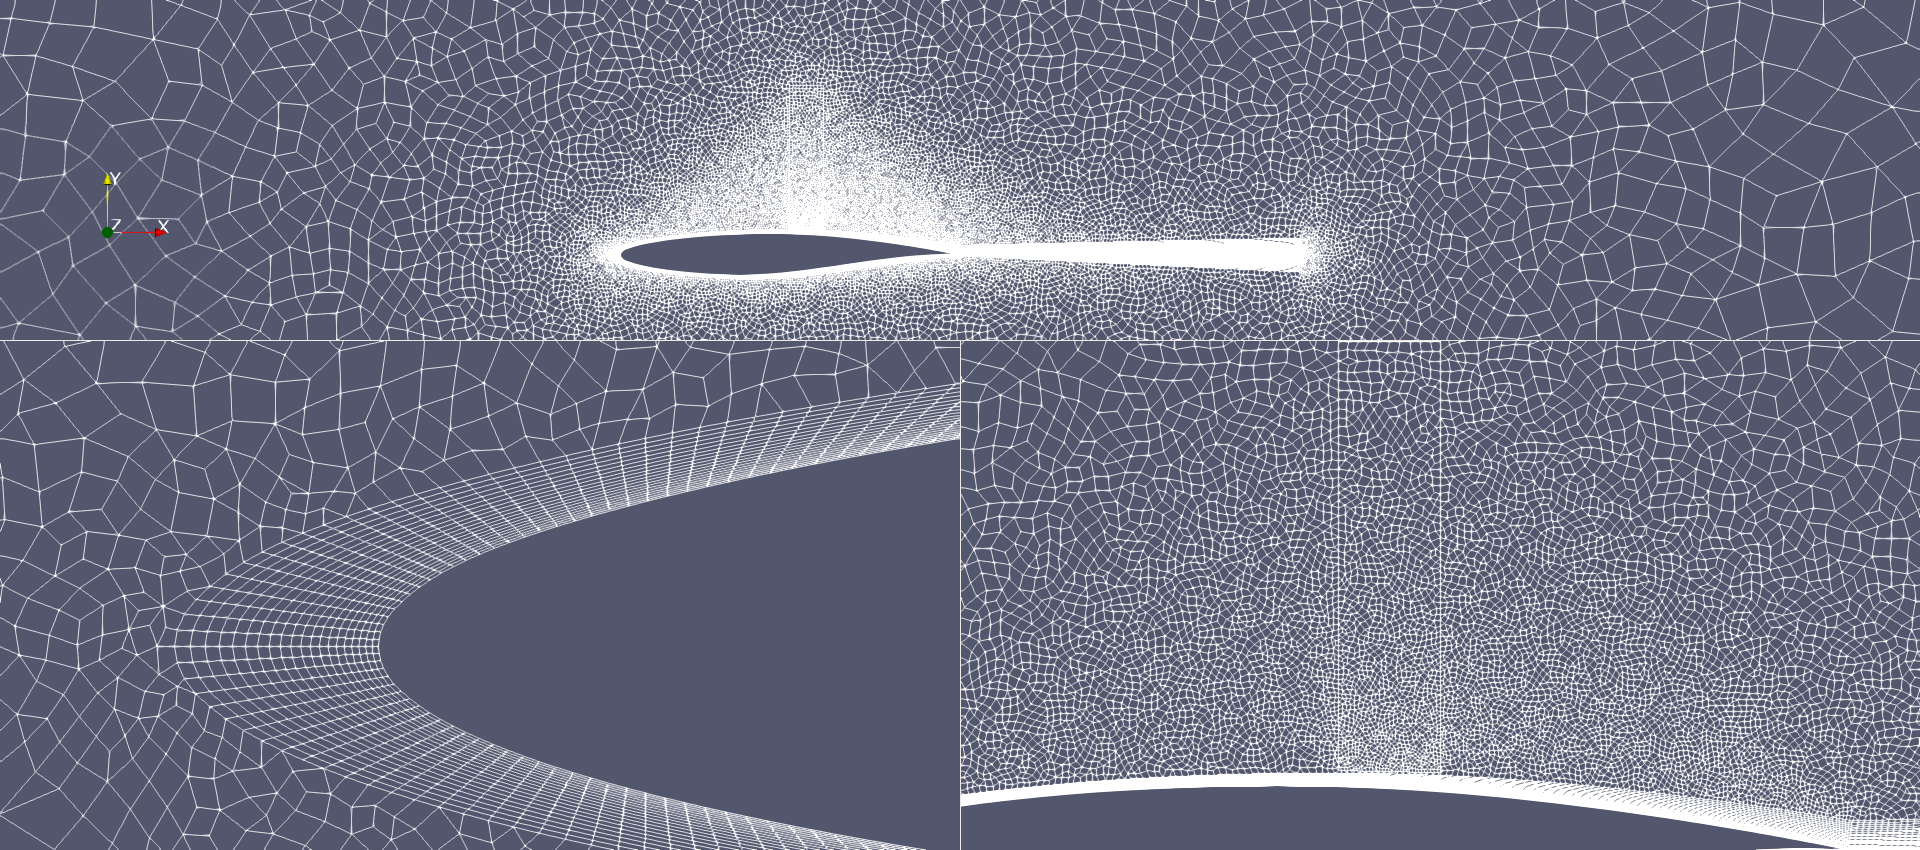
\includegraphics[width=\textwidth]{figures/rae_mesh.png}
          \caption{Mesh for the RAE 2822 test case. Close up on the leading edge and on the expected shock location.}
          \label{fig:rae_mesh}
        \end{figure}

        \paragraph{}
        The model used is the Reynolds Averaged Navier--Stokes equations, or RANS.
        Simply put, every scale of the turbulence is modelled.
        For this case, we decided to use the famous Spalart--Allmaras turbulence model.
        It is well known for being one of the simplest turbulence models, which is fine for us as we want to set up a simple first test case.
        Figure \ref{fig:rae_mesh} shows that the mesh near the wall boundary is not particularly fine, and therefore it is not fine enough to compute the boundary layer.
        It is because this computation uses turbulence wall modelling.
        Such models are known to be troublesome with some more complex turbulence models such as the $k-\epsilon$ model but are used with others such as the one we use here.
        Turbulence wall modelling may be nonconventional in aerodynamic simulations but it is a commonly used feature of our solver, so it is interesting to see how our new method behaves on such test cases.
        The spatial discretisation method is a second-order Finite Volume method, using the HLLC Riemann solver and Multislope method with a Van--Leer slope limiter.
        We also use local time-stepping to speed up the convergence.


      \subsubsection{Analysis of the results}

        \PS{Qu'est-ce qu'on peut regarder pour avoir une différence, flux de chaleur ? Frottement identique sans incidence}

        \paragraph{}
        We are now going to compare the results from the two different simulations.
        It is first worth noting that before trying the JFNK method, we need to start the computation using the traditional method.
        As we explained before, the matrix-free approximation is not ideal to handle discontinuities such as shocks, and a shock is indeed present in this computation.
        Only some iterations are needed, just to start the development of the no-slip boundary layer and approximately place the shock.
        After that, we can restart the computation with the traditional method on one side and with the new method on the other.

        \begin{figure}
          \centering
          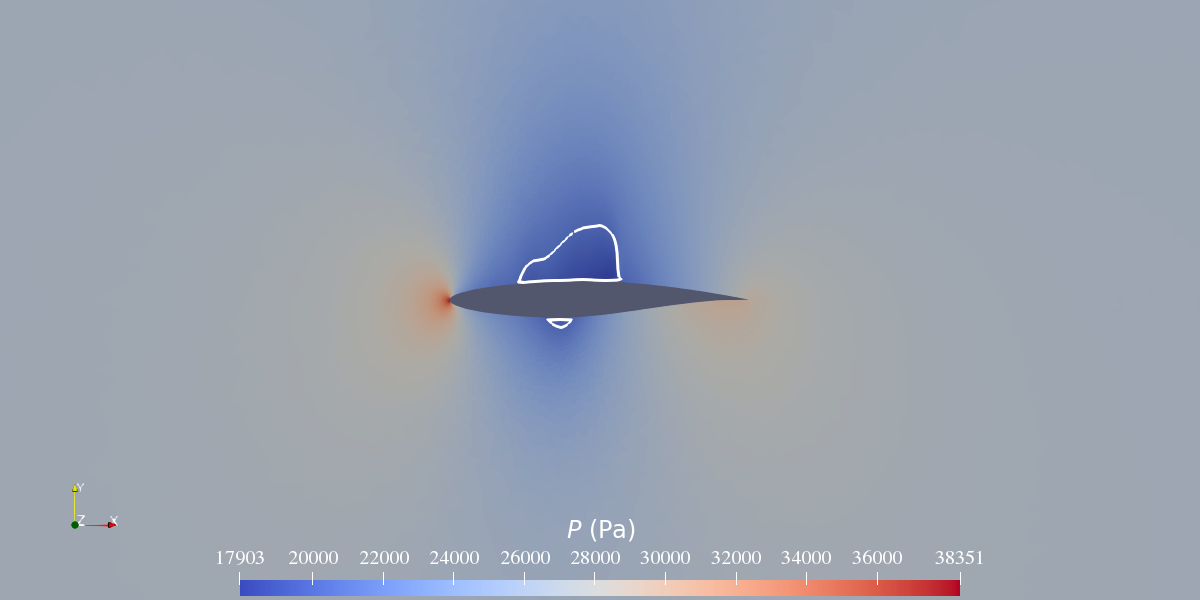
\includegraphics[width=\textwidth]{figures/rae_field.png}
          \caption{Pressure around the RAE 2822 airfoil and sonic $\operatorname{Ma} = 1$ contour.}
          \label{fig:rae_field}
        \end{figure}

        \begin{figure}
          \centering
          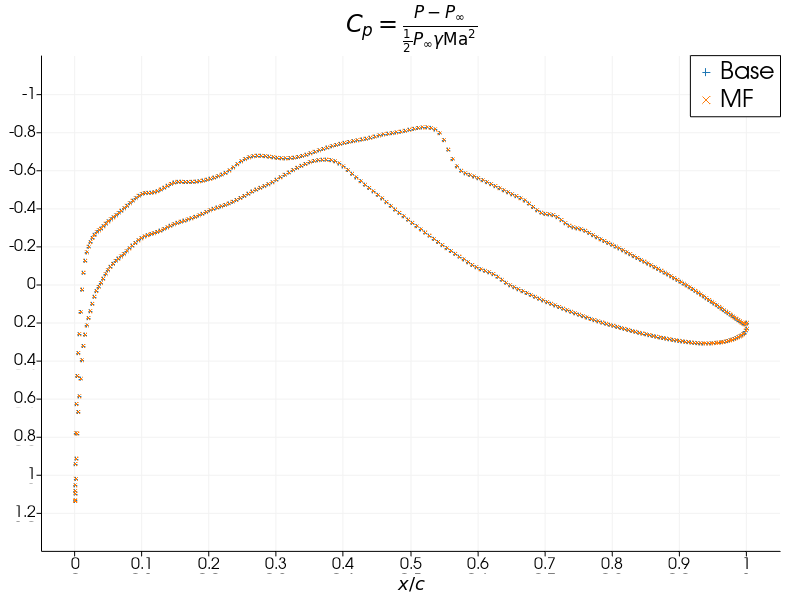
\includegraphics[width=0.7\textwidth]{figures/rae_cp.png}
          \caption{Pressure coefficient around the airfoil for the traditional method (blue) and the JFNK method (orange).}
          \label{fig:rae_cp}
        \end{figure}

        \begin{figure}
          \centering
          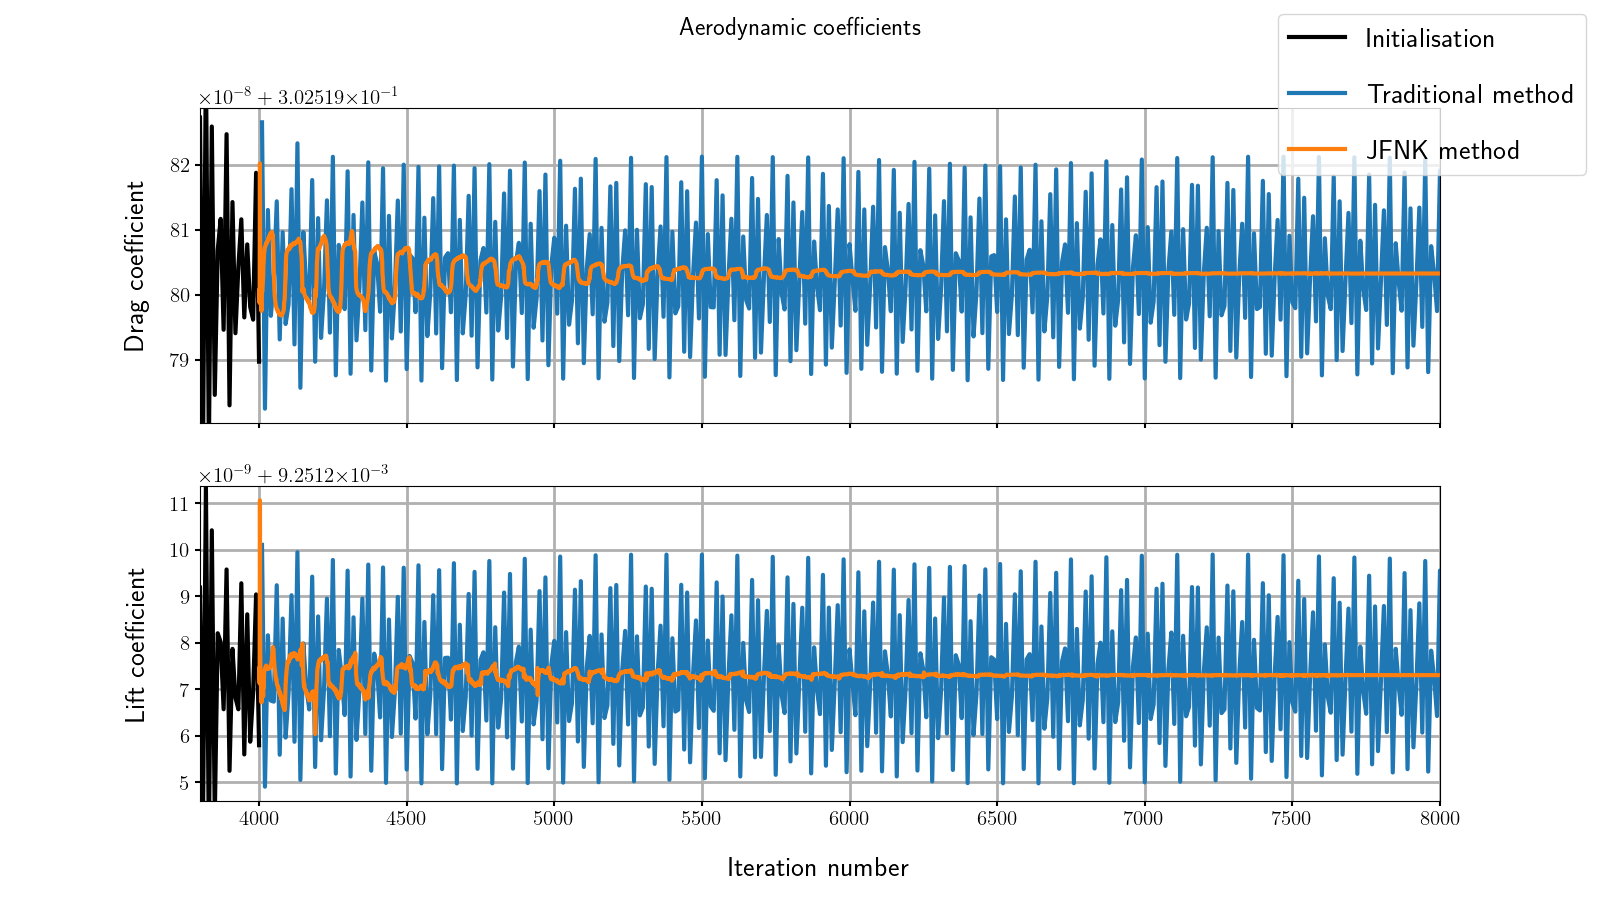
\includegraphics[width=\textwidth]{figures/rae_coefficients.png}
          \caption{Aerodynamic coefficients (lift and drag) for the profile throughout the computation.}
          \label{fig:rae_coefficients}
        \end{figure}

        \paragraph{}
        We can first look at a global image of the flow.
        This is done in figure \ref{fig:rae_field} where we can look at the pressure field near the airfoil.
        In particular, as expected, we see the shock on the upper part.
        The two computations give similar results: they are indistinguishable by just looking at the pressure field.
        This is to be expected as the traditional method gives already satisfying results on such applications.
        We can also look at the pressure coefficient around the airfoil in figure \ref{fig:rae_cp}.
        Once again, the two curves are indistinguishable.
        Finally, we can look at the aerodynamic coefficients, the drag and lift coefficients, throughout the simulation in figure \ref{fig:rae_coefficients}.
        This time, we see an improvement from our method: the coefficients are much more stable, which means the convergence is better with our method.
        The blue curve corresponding to the traditional method struggles to converge and seems to oscillate periodically.
        In comparison, the oscillation of the orange curve is dampened: this corresponds to convergence.
        The scale of the oscillation seen in figure \ref{fig:rae_coefficients} is not significant physically speaking, as it is negligible.
        It shows, however, an issue with the traditional implicit method of the solver CEDRE: it fails to reach proper convergence but it oscillates around the solution.
        The new JFNK method however achieves proper convergence.

        \paragraph{}
        In order to find out if our method did help the convergence of the solver, we need to look at the residuals.
        To define the residuals, we need to go back to the partial differential equation (\ref{eq:pde}) from which we started.
        The residual is in fact the value of the function $\operatorname{F}$ from this equation.
        We can then understand its name for steady problems: it is what is left and still needs to be removed to find a steady solution.
        To decide on the convergence of a steady simulation, we look at this residual norm throughout the computational domain $\mathcal{D}$.
        More precisely, we look at this residual component by component.
        For example, the residual 2-norm associated with the $i$th component is:
        \begin{equation}
          \norm[2]{\operatorname{F}_i} = \int_\mathcal{D} \left| \operatorname{F}_i \right| \mathrm{d}v
        \end{equation}
        and the $\infty$-norm is:
        \begin{equation}
          \norm[\infty]{\operatorname{F}_i} = \max_\mathcal{D} \left| \operatorname{F}_i \right|
        \end{equation}
        In this fluid dynamics application, we can look at the residual norm associated with the conservative variables: the density, the momentum components, the energy and the turbulent variable from the Spalart--Allmaras model $\nu_t$.

        \begin{figure}
          \centering
          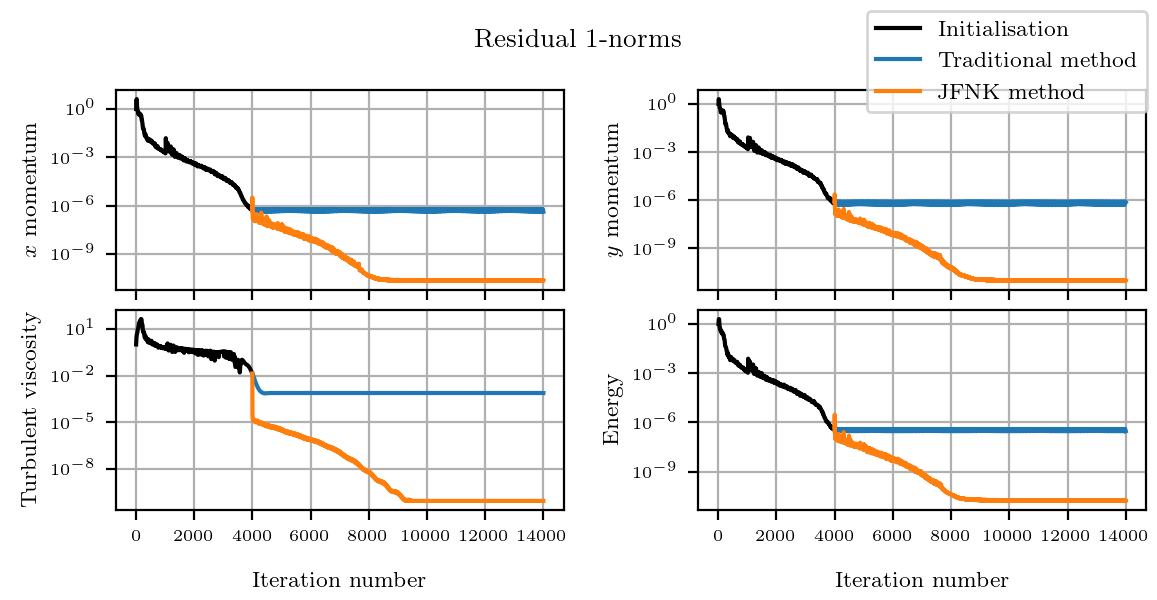
\includegraphics[width=\textwidth]{figures/rae_residuals.png}
          \caption{Residual norms for the two momentum components, energy and turbulent viscosity throughout the computation.}
          \label{fig:rae_residuals}
        \end{figure}

        \paragraph{}
        Figure \ref{fig:rae_residuals} shows the residual norms from our two computations.
        The gain from using the JFNK method appears clearly.
        The final residual norm is much smaller for each and every conservative component.
        This means that the Jacobian-Free Newton--Krylov method is able to reach a better convergence level than the traditional method.
        In other words, the better Jacobian matrix approximation from our new method leads to a better convergence than the older poor approximation.

        \paragraph{}
        In this first test case, we looked at the residual norms as the fields computed by both methods were almost identical.
        Moreover, our method was even able to reach better convergence levels.
        This validates our method on a first simple case, albeit with turbulence modelling and a shock.


    \subsection{Turbulent transonic airfoil with boundary layer resolution}
    \PS{MAYBE ?}

      \subsubsection{Definition of the test case}

        \paragraph{}
        The previous case uses a mesh that is too coarse to resolve the boundary layer but instead uses a turbulent wall mode.
        It is representative of CEDRE applications, but not of actual applications from the aerodynamic community.
        The RAE 2822 airfoil is often used for turbulence model validations, but computations in the field prefer to use a finer mesh to resolve the boundary layer.
        This is what we present next.
        The new mesh, shown in figure \ref{fig:rae_mesh_fine} is clearly different.
        It is a 3D mesh, which is in fact a 2D mesh that was extruded on 6 cells in the $y$ direction.
        We set a periodicity between the two sides of the domain.
        The mesh is made of 198144 cells whereas the previous RAE 2822 mesh was only made of 36541 cells.
        With these additional cells, this mesh is able to be fine on the wall boundary condition as is seen in figure \ref{fig:rae_mesh_fine}.
        This means that we do not need to use the turbulent wall model we used in the previous test case.
        We still use the Spalart--Allmaras one equation turbulence model.
        The scale of the mesh is the same: the chord is still equal to $1\si{\meter}$.

        \begin{figure}
          \centering
          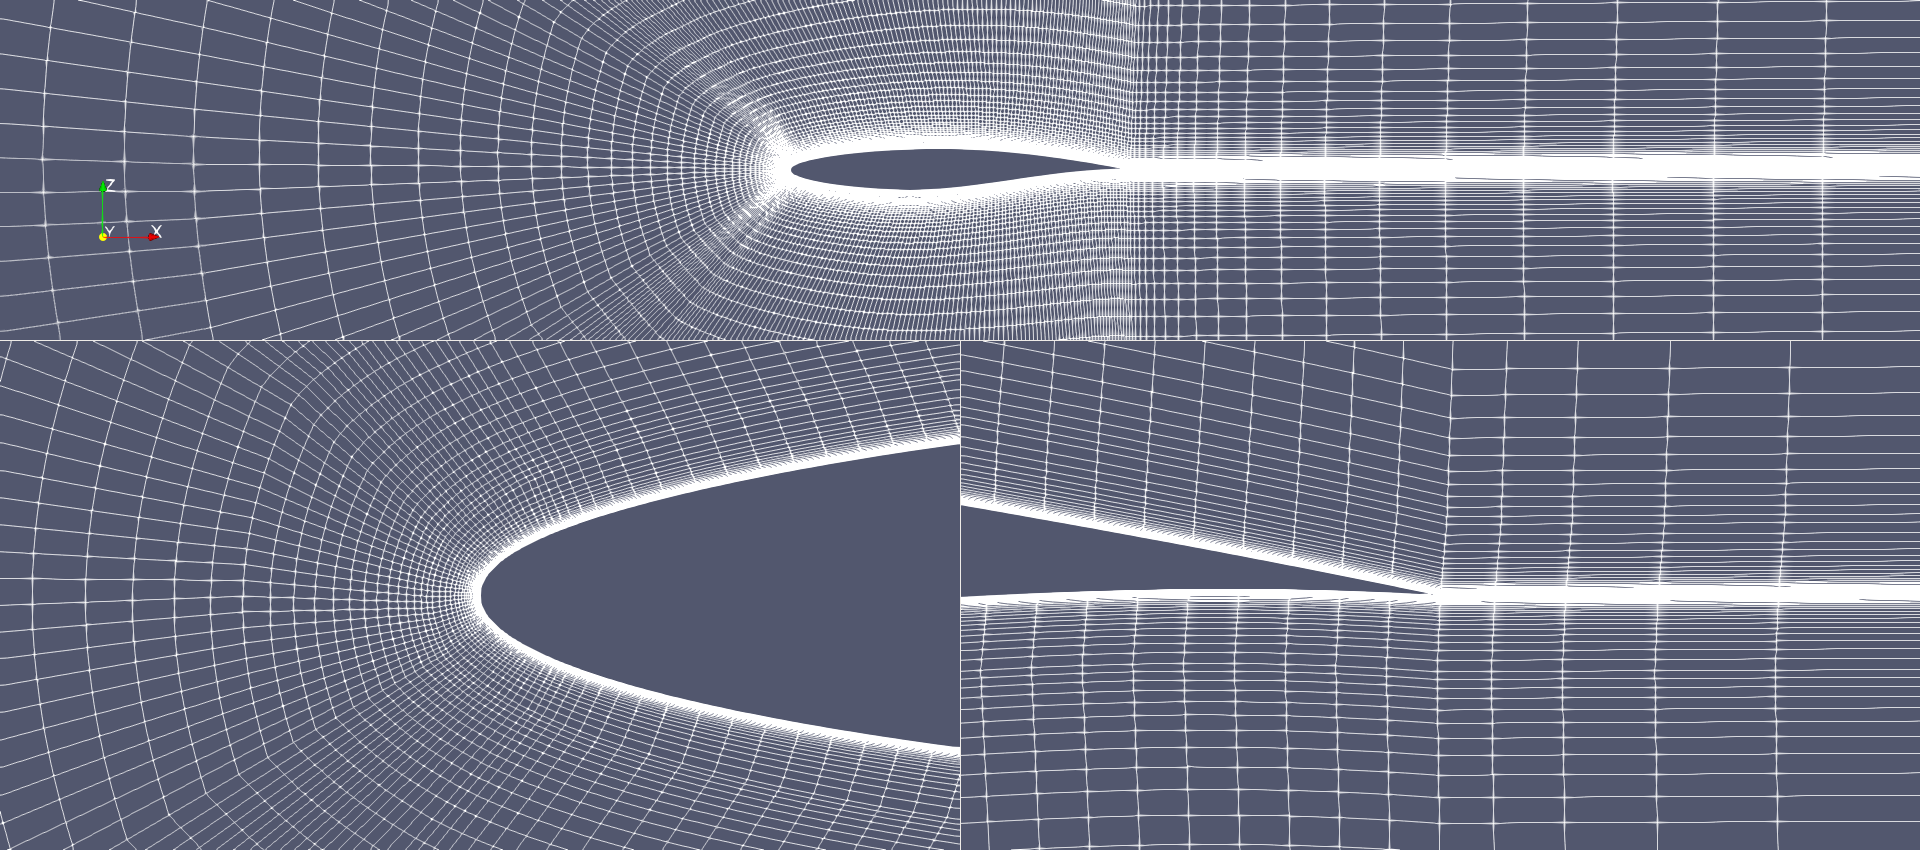
\includegraphics[width=\textwidth]{figures/rae_mesh_fine.png}
          \caption{Finer mesh for the RAE 2822 test case. Close up on the leading and trailing edges.}
          \label{fig:rae_mesh_fine}
        \end{figure}

        \paragraph{}
        The flight conditions are also modified to match some existing experimental conditions: the AGARD-AR-138 experimental database.
        We take a Mach number equal to 0.729, and the angle of attack is $2.31\si{\degree}$ with a Reynolds number of \num{6.5e6}.
        \PS{TODO}


    \subsection{Hypersonic reactive sphere}

      \paragraph{}
      The second application we selected to compare the Jacobian-Free Newton--Krylov with the traditional one is the computation of the flow around a hypersonic solid sphere.
      Because of the high energy of the surrounding flow, the air molecules can separate and even form a plasma.
      The hypersonic reactive sphere is a well-known case, for both experimental \cite{Lobb1964} and numerical studies \cite{DobrovGimadievKarpenkoEtAl2022}.
      This is a simple yet representative test case of CEDRE applications.
      It then makes a lot of sense to analyse our new method on it.

      \subsubsection{Definition of the test case}

        \PS{AVEC OU SANS CHIMIE ?}

        \begin{figure}
          \centering
          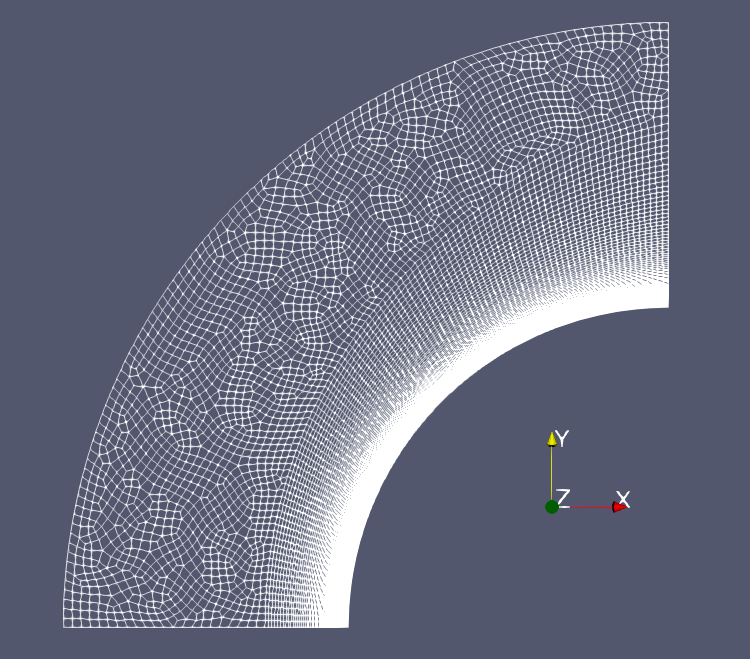
\includegraphics[width=0.6\textwidth]{figures/sphere_mesh.png}
          \caption{\PS{TODO: c'est pas le bon maillage}}
          \label{fig:sphere_mesh}
        \end{figure}

        \paragraph{}
        The 2D mesh is shown in figure \ref{fig:sphere_mesh}.
        It is a regular mesh made of quadrangles, with refinement in the radial direction at the wall boundary and at the expected shock location.
        The refinement at the wall boundary helps to compute more precisely the physical phenomena that happen at said boundary.
        The refinement at the shock is a requirement of the spatial discretisation methods.
        In order to get a clean and slim shock, the cells near the shock must have a high aspect ratio.
        Otherwise, artificial vorticity is created when going through the shock, which will give wrong results downstream. \PS{c'est bien pour ça ?}
        This expected shock location is obtained from a previous computation, made with a coarser mesh.
        This mesh is used in a 2D axisymmetric computation to get the flow around a 3D solid sphere.

        \paragraph{}
        The solid sphere is modelled by an isothermal wall boundary condition.
        This is a representative choice as well, as the heat flux going through the wall is one of the main interests of such computation.
        Moreover, as it depends on the derivatives of the flow variables, it is usually harder to get a correct value for the heat transfer.
        A better convergence will lead to better derivatives, which will lead to better physical results for such case users.
        No turbulence model is used, as the flow is mostly laminar.

        \paragraph{}
        The main feature of this test case is that it simulates a hypersonic flow.
        At the left, the input boundary condition feeds air at Mach 15.
        This will induce a strong shock, meaning a strong discontinuity in the flow.
        As this is a typical application of our solver, it is of importance to us that the new method behaves well with such flow features.
        When going through a strong shock, the temperature of the flow will increase a lot.
        The flow is made of air, or a mixture of 77\% \ce{N_2} and 23\% \ce{O_2}.
        At the high temperature they reach after the shock, the molecules can decompose into \ce{N}, \ce{O}, and \ce{NO}.
        They can even get ionised.
        In our model, we end up using 11 possible species: \ce{N_2}, \ce{O_2}, \ce{N}, \ce{O} and \ce{NO}, the corresponding cations \ce{N_2^+}, \ce{O_2^+}, \ce{N^+}, \ce{O^+} and \ce{NO^+} and the electrons \ce{e^-}.

        \begin{figure}
          \centering
          % 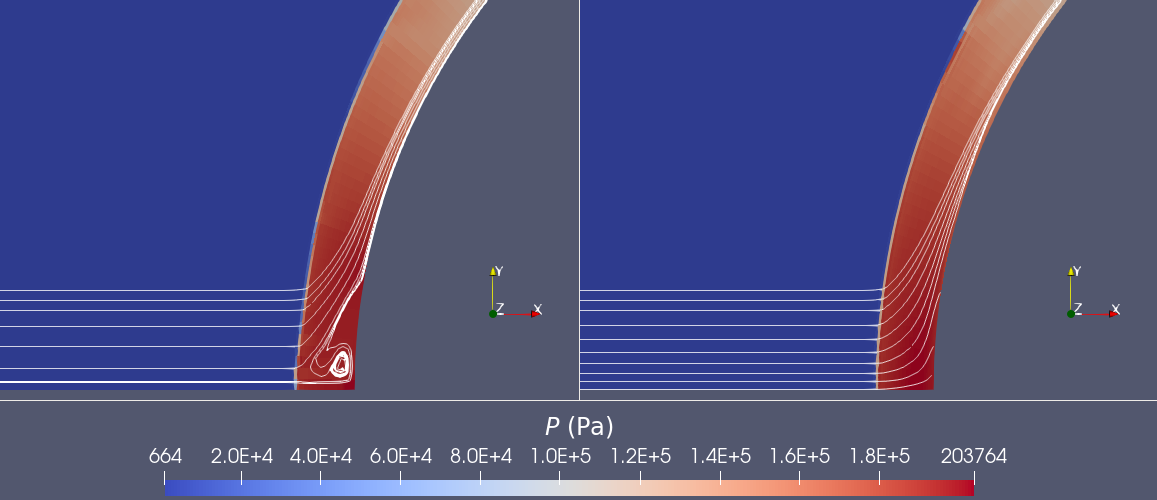
\includegraphics[width=0.6\textwidth]{figures/sphere_carbuncle.png}
          \caption{\PS{TODO} Streamlines near the sphere for two Riemann solvers.}
          \label{fig:sphere_carbuncle}
        \end{figure}

        \paragraph{}
        We argued previously that our solver is quite complex and that it makes it hard to do correct computations for non-experimented users.
        This hypersonic reactive sphere is a perfect example of this statement.
        Even if this case looks simplistic, it should not be taken lightly.
        While using unfit spatial discretisation methods, we ended up with a well-known problem of a such simulation called carbuncle \cite{MacCormack2013}.
        This phenomenon does not come from physics but is solely due to numerical methods.
        It is shown in figure \ref{fig:sphere_carbuncle}.
        Simply put, it creates a recirculation bubble downstream of the shock, near the stagnation point.
        This bubble tends to push the shock farther from the sphere, and modify greatly the heat flux at this location.
        The choice of the Riemann solver ended up being the key element to getting rid of this undesirable effect: there is no recirculation with the AUSM+ scheme.
        There are other pitfalls regarding this test case in CEDRE.
        For example, the user can choose whether to interpolate the mass fraction $y_i$ for the species at the cell interfaces for the MUSCL scheme or the \PS{mass concentration} $\rho y_i$.
        Choosing the default option leads to nonconverging residuals no matter the time integration method.
        Indeed, this default option is recommended when running simulations with multiple phases, with significant variations in the density.
        Because CEDRE is made to solve a large variety of problems, it has a lot of methods that come with a lot of parameters, so even a simple simulation such as this one requires a lot of knowledge if a good convergence is required.

        \paragraph{}
        This test case is a typical application of CEDRE, as opposed to the previous one which focuses more on the aerodynamic properties.
        Indeed CEDRE does not try to be a pure aerodynamic solver but a multiphysics one, equipped to solve high-energy problems.
        Reentry phenomena are therefore in the scope of our solver.
        Any improvements coming from our method on such applications would benefit a lot of CEDRE users on their applications.


      \subsubsection{Analysis of the results}

        \paragraph{}
        Once again, a first computation is done using the more robust traditional method.
        Indeed, the flow in the first cell against the sphere and the symmetry axis is initialised with a Mach number of 15 going straight into the wall.
        The matrix-free approximation struggles with such stiff initialisations, which is why we must start the computation with another method, just until the shock has started to detach from the wall.
        Practically this amount to just a few iterations, compared to the number required to achieve convergence.

        \paragraph{}
        We first look at the different fields from the two computations.
        Once again they are similar and we will use the residuals to compare them, but we can check we are indeed computing the features of interest.
        In figure \PS{TODO}, we see that the shock is present and that it falls as expected in the refined region.
        We see in figure \PS{TODO} the mass fraction of the various species downstream of the shock, which means we are actively computing the chemical features of the flow, as expected.
        \PS{Comparaison distance corps shock avec \cite{Lobb1964} ?}

        \paragraph{}
        Once again, we will not see any difference between the two results if we look at the \PS{standard} quantities.
        We might see them if we look at quantities that depend on the derivatives of the flow variables, and that is why we will look at the \PS{heat transfer coefficient} at the wall.
        The results are displayed in figure \PS{TODO}.
        \PS{A VERIFIER MAIS DE MEMOIRE :}
        Unfortunately, there is not much difference to be seen between the two methods: they both produce the same heat transfer coefficient.
        We also see an issue: the heat flux should be maximum at the stagnation point, but we see in figure \PS{TODO} that it is not, and the slope of the heat transfer coefficient is not null at the stagnation point in both of our simulations.
        This shows an inaccuracy of the solver.
        However, as we will show next, the time integration is able to find the correct converged steady solution.
        Therefore this inaccuracy comes from the spatial discretisation method.
        The results are not accurate from a physical analysis perspective, but for us, the methods both work fine: they find the expected steady solution, albeit it is not the expected physical one.

        \paragraph{}
        The advantage of the new method appears when we look at the residuals: we see in figure \PS{TODO} that the new method gives a better convergence.
        The difference between the traditional method and the new one is that the traditional method uses the Jacobian matrix of the first-order spatial discretisation method, whereas the new one approximates the true Jacobian matrix using the approximation (\ref{eq:matrix_free}).
        We decided to test this.
        Because this simulation does not use complex models, the poor approximation used in the traditional model should give the Jacobian matrix of the first-order scheme.
        If we use the approximation (\ref{eq:matrix_free}) but use the first-order evaluation of $f$, then we should also get the same Jacobian matrix.
        We look at the residual norms from this method, which we can call the first-order JFNK method, and we see in figure \PS{TODO} that it is indistinguishable from the residual norms from the traditional method.
        It first validates the development of the matrix-free approximation, and that the unbridle method should then use the actual second-order Jacobian matrix.
        It also confirms that the traditional method uses the Jacobian matrix of the first-order spatial discretisation method.
        Finally, it validates the choice of $\varepsilon$ and the matrix-free approximation, as it is able to give the same result as when we use the Jacobian matrix.

        \paragraph{}
        When we use the new method, using the true function $f$ with a second-order, we see that we can get a much smaller residual norm.
        The only difference between the two methods is that the traditional one uses the Jacobian matrix of the first-order spatial discretisation method, but the JFNK method takes into account the MUSCL reconstruction when using the Jacobian matrix.
        Because it uses a better Jacobian matrix in the linear solve, it gives a better solution to the nonlinear solve, which gives in turn a better time integration.
        It confirms that using a better Jacobian matrix helps the overall convergence when solving steady problems and validates the choice of the Jacobian-Free Newton--Krylov method.


    \paragraph{}
    In a previous part, we suggested that the poor quality of the Jacobian matrix used in our solver was an obstacle to achieving good convergence.
    We then proposed an improvement: the Jacobian-Free Newton--Krylov method using the matrix-free approximation (\ref{eq:matrix_free}).
    We compared this new method with the traditional one on two simple yet representative applications of our solver.
    This comparison showed that indeed, using a better Jacobian matrix leads to a lower residual norm.
    The new method can be useful when looking at quantities that require precise convergence, for instance, the derivatives of the flow variables.
    However, the main drawback of this new method is its computational cost.
    This cost is not inherent to the method but comes from our solver properties as was discussed previously.
    The recommended usage is then to start a computation using the inexpensive traditional method, and then achieve better convergence using the more precise yet more expensive new method.


  \section{Utilisation de la formulation sans matrice sur un nouveau modèle de fluide}

    \paragraph{}
    In the previous section, we compared the new Jacobian-Free Newton--Krylov method to the traditional method that uses the first-order Jacobian matrix.
    This first-order matrix is easily computed for the usual Navier--Stokes equations.
    But as CEDRE is under constant development, new models are added in order to handle more finely various multiphysics phenomena.
    For example, a new model was recently added to better handle multiphasic flows \cite{Cordesse2020}.
    Adding a new model amount to writing the function $\operatorname{F}$ from equation (\ref{eq:pde}), or equivalently $\operatorname{G}$ from equation (\ref{eq:ode}).
    Usually, the development of this function is straightforward as it is given explicitly from the equations.
    However, the development of the Jacobian matrix is much more difficult.
    This is why the new models can not compute Jacobian matrices, and therefore can not use implicit methods.
    The Jacobian-Free Newton--Krylov method is then a nice way to use implicit methods as it does not require the Jacobian matrix.
    Because the matrix-free approximation is written in a generic fashion, it can be used on any fluid model.
    In the following, we will use the JFNK method on a new fluid model that does not have an available Jacobian matrix and therefore can not use traditional implicit methods.


    \subsection{Multi-TEmperature model}

      \paragraph{}
      The new model we will use is called the \emph{Multi-TEmperature model}, or MTE.
      Its difference from the traditional Navier--Stokes model is that it allows for a thermodynamic non-equilibrium of some flow components.
      A particle has multiple degrees of freedom: translation, rotation and vibration.
      In more traditional models, it is assumed that all modes are at equilibrium, and they are grouped in what we call energy.
      We can define a time constant for each energy mode that corresponds to the number of collisions that are required to get to the equilibrium.
      A few collisions are required for translation modes, and about ten for rotation modes.
      This gives a small time constant of order $10^{-9}\si{seconds}$.
      For vibration modes, however, up to \num{20000} collisions are required.
      The corresponding time constant is significantly larger, and there may be regions where there can be a disequilibrium between vibrational energy on one side and translation and rotation energy on the other.
      The energy of such components can no longer be described with a single temperature.
      As electrons are much lighter, they move more than the other heavier flow components.
      Their transitional energy and the transitional energy of other components can not be described with the same temperature.
      With the new Multi-TEmperature model, the flow components may be divided into three classes:
      \begin{itemize}
        \item the ones that always are at the equilibrium
        \item the ones that may be at vibrational disequilibrium
        \item the electrons that are handled separately from the other heavy component.
      \end{itemize}

      \paragraph{}
      To account for the disequilibrium, the Navier--Stokes equations (\ref{eq:ns}) are modified into the following, in conservative form.
      \begin{equation}
        \left\{\begin{alignedat}{5}
          &\partial_t\left(  \rho_s  \right) &&+ \nabla\cdot\left(  \rho_s \vec{u}  \right) &&=
            \nabla\cdot\bigl( \rho D_s \nabla y_s\bigr) + \dot \omega_s \\[10pt]
          %
          &\partial_t\left(  \rho \vec{u}  \right) &&+ \nabla\cdot\left(  \rho \vec{u} \otimes \vec{u}  +  \left(p + p_e\right) \mat{\operatorname{Id}}  \right) &&=
            \nabla\cdot\biggl(
              \mu \left(\nabla \vec{u} + \nabla \vec{u}^T\right)
              - \frac{2}{3} \mu \left(\nabla \cdot \vec{u} \right) \mat{\operatorname{Id}}
            \biggr) \\[10pt]
          %
          &\partial_t\left(  \rho_m e_{v,m}  \right) &&+ \nabla\cdot\left(  \rho_m e_{v,m} \vec{u}  \right) &&=
            \nabla\cdot\bigl(
              \lambda_{v,m} \nabla T_{v,m}
              + \rho e_{v,m} D_m \nabla y_m
            \bigr) \\
            &&&&& \phantom{= {}} + S^{v-t}_m + S^{v-v}_m + S^{v-e}_m + \dot \omega_m e_{v,m} \\[10pt]
          %
          &\partial_t\left(  \rho_e e_e  \right) &&+ \nabla\cdot\left(  \left(\rho_e e_e + p_e\right) \vec{u}  \right) &&=
            \nabla\cdot\bigl(
              \lambda_e \nabla T_e
              + \rho h_e D_e \nabla y_e
            \bigr)
            + \vec{u} \cdot \nabla p_e \\
            &&&&& \phantom{= {}} + S^{e-t} + S^{e-r} + S^{e-v} + \dot \omega_e e_e \\[10pt]
          %
          &\partial_t\left(  \rho E  \right) &&+ \nabla\cdot\left(  \left(\rho E + p + p_e\right) \vec{u}  \right) &&=
            \nabla\cdot\Biggl(
              \lambda_{eq} \nabla T
              + \sum_m \lambda_m \nabla T_m
              + \lambda_e \nabla T_e \\
              &&&&& \phantom{=\nabla\cdot\Biggl(} + \mu \left(\nabla \vec{u} + \nabla \vec{u}^T\right) \vec{u} - \frac{2}{3} \mu \left(\nabla \cdot \vec{u}\right) \vec{u} \\
              &&&&& \phantom{=\nabla\cdot\Biggl(} + \rho \sum_s h_s D_s \nabla y_s
            \Biggr)
        \end{alignedat}\right.
      \end{equation}
      What we see first is that the equations of this physical model are more complex compared to the standard Navier--Stokes equations.
      We notice there are multiple energies corresponding to the multiple temperatures: $e_e$ the energy of the electronic gas, $e_{v, m}$ the vibrational energy for each flow component that may be at disequilibrium, and $E$ the total energy.
      It increases the number of conservative variables.
      The variables $y$ correspond to the mass fraction of the different flow components.
      The source terms $\omega$ correspond to chemical production or decay.
      The source terms $S$ correspond to the energy transfers between the different energy modes.
      The details of those terms can be complex and are not discussed here as it is not the subject of this thesis, but can be found in \cite{Soubrie2006}.
      A noticeable feature of this model is the presence of a nonconservative term in the conservation equation of the electrons' energy: $\vec{u} \cdot \nabla p_e$.
      This term is due to the effect of the electric field.
      This is a known issue of this model, as the Finite Volume method handles better conservative terms.
      Some work tried to transform this equation into a conservative one by using the electronic entropy instead of energy but by neglecting dissipation terms concerning the electrons \cite{CoquelMarmignon1995}.
      However, this simplification can lead to inaccuracy in the physical result, and it appears that using the nonconservative formulation is necessary to get physically accurate results \cite{Soubrie2006, KimGuelhanBoyd2012}.
      Not to go into too much detail, such models that account for thermodynamic disequilibrium are still under discussion as of today \cite{BlancoJosyula2020}.

      \paragraph{}
      The Multi-TEmperature model allows for non-equilibrium between the vibrational mode of the flow components, the electronic energy and the total energy.
      Taking this non-equilibrium into account helps to compute more precisely physical quantities such as the electronic density, which can be useful for magnetohydrodynamics applications for example.
      It gives a better prediction of shock layer radiation with a better representation of the population of energy states which helps the simulation of radiation cooling or the computation of wall heat fluxes.
      This model is most interesting on reentry problems, as there is indeed some non-equilibrium downstream of the strong shocks that appear on such problems.
      Taking the non-equilibrium into account can change the flow downstream of the shock and on the solid wall, and give more precise temperatures and chemical compositions.
      Generally speaking, the Multi-TEmperature model gives more precise results than the standard Navier--Stokes model on fast flow with low relative density where there may be some thermodynamic non-equilibrium, such as reentry problems or problems with the strong expansion of a plume.


    \subsection{Hypersonic reactive sphere}

      \paragraph{}
      The hypersonic sphere test case is a perfect fit for the Multi-TEmperature model.
      There is some thermodynamic non-equilibrium in the region downstream of the shock, because of its intensity.
      Unfortunately, the Jacobian matrix for the new MTE model is not currently available.
      This limits the MTE model users to explicit time integration methods, and therefore small time steps for stability reasons.
      As they deemed explicit time integration too slow, they wanted to use the newly implemented Jacobian-Free Newton--Krylov method for their simulations.
      We will show in the following another interest of the matrix-free approximation: it allows for implicit time integration methods despite having no Jacobian matrix.
      The goal here is to be able to get a steady solution to the problem as fast as possible for the user.
      Initially, the MTE model users were using a second-order Runge--Kutta method: the Midpoint method.
      We will compare the JFNK method to this reference method, and we will look in particular at how much time is required from the user to get to a physically satisfying result.


      \subsubsection{Full reactive model}

        \paragraph{}
        For the first step of our analysis, we will use the most complete physical model.
        We use the same 11 flow components as before: \ce{N_2}, \ce{O_2}, \ce{N}, \ce{O} and \ce{NO}, the corresponding cations \ce{N_2^+}, \ce{O_2^+}, \ce{N^+}, \ce{O^+} and \ce{NO^+} and the electrons \ce{e^-}.
        We of course use the Multi-TEmperature model, and we consider that \ce{N_2} and \ce{O_2} may be at vibrational disequilibrium.
        Other components may in fact also be at disequilibrium and we could take them into account but the computational cost increase is not worth it.
        As they are less present, and they quickly get to the equilibrium relatively to \ce{N_2} and \ce{O_2}, accounting for their disequilibrium would not be significant in the results \cite{Park2006}.
        This amount to having four temperatures to describe the flow: $T_e$ for the electrons, $T_{v, \ce{N_2}}$ and $T_{v, \ce{O_2}}$ for the vibration modes of \ce{N_2} and \ce{O_2}, and $T$ for the total energy.

        \paragraph{}
        As before, the Jacobian-Free Newton--Krylov method needs some help at the beginning.
        This is why we start the computation with some iterations of the Midpoint method.
        Then, we continue the computation with the JFNK method using the first-order Finite Volume method, to quickly get a good enough approximation of the expected solution.
        Finally, to get a finer result, we end the simulation using the second-order spatial discretisation method.
        We use local time-stepping based on the CFL number.
        We can not use preconditioners that use the matrix, so the only one available is the diagonal preconditioner based on the cell volumes.
        It is not ideal as it is extremely simple, and some physics-based preconditioner would be preferable \cite{KnollKeyes2004} but none were available to us at the time.
        The spatial discretisation method used is the Multislope method, as it appears more robust than the $k$-exact method with the Multi-TEmperature model.

        \paragraph{}
        The goal of this thesis is not the physical analysis of this test case so it will be left out, but according to the MTE model users, the results are in agreement with the literature. \PS{Ca va ?}
        We show in figure \PS{TODO} the various temperatures along the symmetry axis.
        This justifies the use of the Multi-Temperature model: the region downstream of the shock is indeed in a thermodynamic non-equilibrium state.
        \PS{Hypothétique : Comparaison AET MTE}

        \paragraph{}
        We will also look at the residuals for this analysis.
        But this time, we will not be using the number of iterations as the $x$-axis as it will be unfair to the explicit method.
        Indeed the cost of one iteration is a lot smaller for the explicit method than for the implicit JFNK one.
        What matters to us and a typical user is not the number of iterations but the time spent waiting for the result.
        It is called the elapsed real time or wall-clock time.
        As we will run our computations each time in the same parallel environment, with a fixed number of CPU cores, the elapsed time is proportional to the CPU time.
        The $x$-axis will then be the CPU time: the actual time it took to get to the current residual.

        \paragraph{}
        Figure \PS{TODO} shows the residual norms for the two computations.
        The leftmost black curve corresponds to the initialisation: a few iterations of the explicit time integration method.
        From then we can continue the computation with the Midpoint method on one side and the Jacobian-Free Newton--Krylov method on the other.
        We see that the residual norm obtained with the JFNK method is lower than its explicit counterpart.
        Indeed, the explicit method is limited to small time steps because of the shock and the stiff reactive model.
        \PS{C'est sûr ça ? Parce que l'explicite n'a même pas l'air de bouger ...}
        The implicit method however is not.
        The fact that the implicit method can use larger time steps is not new, but with this specific model, it was not possible to use implicit methods until we added the matrix-free approximation.
        The JFNK method even ends up being cheaper in terms of CPU time.
        This means that for a user, it is faster to use the newly implemented Jacobian-Free Newton--Krylov method than to use explicit methods.
        Our method gives a better alternative to users working on problems with the Multi-TEmperature model.


      \subsubsection{Simplified reactive model}

        \paragraph{}
        The equations concerning electrons in the Multi-TEmperature model bring a lot of issues.
        It is because the quantity of free electrons is usually relatively small when compared to other flow components.
        It can lead to numerical instabilities or cause other problems.
        As the equations hold everywhere in the numerical domain, they hold in particular in areas without free electrons, upstream of the shock in our hypersonic sphere for example.
        The question one must ask is then how to compute quantities such as the electronic temperature $T_e$ where there are no free electrons.
        We will not go into such implementation details as it goes beyond the scope of this work, but the point is that having electrons is quite troublesome for numerical methods.
        According to users that work on such reentry applications, it is not always useful to compute fluid ionisation.
        We explained why it might be crucial for some simulations, but when we do not look at the electrons, their effect on other quantities is almost negligible.
        Those users said that \PS{"ça craint de dire "il a dit que" ?"} it is acceptable, meaningful and still useful to do the same simulation but ignoring electrons.
        It is done by considering only the chemical components \ce{N_2}, \ce{O_2}, \ce{N}, \ce{O} and \ce{NO}.

        \paragraph{}
        We decided to do the same comparison as before but this time with the simplified reactive model.
        We once again start the computation with a few iterations of the Midpoint method and use that as a common initialisation.
        Then, we compare the explicit method with the Jacobian-Free Newton--Krylov method.
        We show the corresponding residual norms in figure \PS{TODO}, while still using the CPU time as the $x$-axis.
        The result is similar to the previous one, except it is even more in favour of the JFNK method.
        The implicit method reaches much lower residual norms than the explicit one.
        With the full reactive model, the limiting factor for the implicit method came from the stiffness due to the electrons.
        Without them, the convergence is significantly faster.
        The time step for the explicit method however is under the same limitations with both reactive models.
        The gain in CPU time is then huge, in favour of the JFNK method.
